%\chapter{Alfred Tomatis}


\section{Le test d'écoute de Tomatis}


Selon son ouvrage,\footnote{\emph{Éducation et
    Dyslexie}\autocite{tomatis:education}}la représentation graphique tirée du 
 ``\emph{Hearing Test}'' distingue l'écoute générale de l'auto-écoute avec l'observation des modifications et des évolutions des courbes
  aériennes et osseuses.\footnote{<<\,Considérations sur le test d'écoute\,>>. Propos
  	recueillis au cours du \textsc{iii}\ieme\ congrès international
  	d'audio-psycho-phonologie (Anvers 1973) lors d'un entretien
        avec B. Auriol. \autocite{auriol_stress}}





Tomatis a défini la «courbe d'écoute idéale», courbe qui correspond à l'oreille absolue
des chanteurs et des musiciens,  avec  le ténor italien Enrico
Caruso (1873--1921) dont il a analysa la voix à partir des
enregistrements sur disque. Caruso représentait la courbe auditive
optimale dont il décida de se référer. C'est une courbe ascendante entre 500 et 2000
Hz qui correspond à une pente d\textquoteright environ 6 à 18 db/octave,
puis un dôme entre 2000 et 4000 Hz et ensuite une légère descente. 

      Sur le plan de la physique pure, elle indique les réponses de l'oreille
lorsque celle-ci fonctionne bien. Elle répond en fait à la courbe
de Wegel dite ``courbe en citron", inversée.\footnote{
		Voir l'annexe \ref{acoustique} p. \pageref{acoustique}
		 pour cette partie technique.}.

               

L'acquisition de cette courbe idéale correspond à l'\textsl{harmonisation}
du jeu de deux muscles de l'oreille moyenne. Celui-ci 
permet de régler en permanence la pression interne au niveau du
labyrinthe.

Sur le plan du test d'écoute, on évaluera et visualisera la différence
graphique selon la courbe dite 
idéale. Lorsque la forme de
courbes est continue et parallèle et qu'il n'y a pas de distorsions, on parle d'harmonie. L'harmonie
est la représentation de la régulation des émotions, l'équilibre entre
une écoute
intérieure et extérieure.

Ces paramètres sont importants et nous reviendrons plus en détail sur
la passation du test d'écoute.
%\enquote{\emph{L'oreille a un
%psychisme\autocite[{tomatis:loreille}.}} 

Lorsque l'interprétation des informations transmises à l'oreille est
erronée, il y a une 
\textbf{distorsion d'écoute}, liée au dysfonctionnement
de ces deux muscles dont le rôle est de permettre l'arrivée
harmonieuse du son dans l'oreille interne, puis au cerveau. Car, lorsque
le message sensoriel est altéré, le cerveau se protège en déclenchant
des mécanismes d'inhibition de l'écoute, traduit souvent par un relâchement de
ces plus petits muscles du corps humain. Ce potentiel acquis à
la naissance peut s'altérer avec les difficultés inhérentes à
la vie et la protection recherchée (inconsciemment) contre certaines agressions et le subterfuge le plus
efficace qu'a élaboré le cerveau est
d'introduire des distorsions, comme citées plus haut. De même, constate B. Auriol
les différents maux comme l'otite, l'eczéma, l'hyper
ou hypo sécrétio de sébum sont liés à l'interaction de sons refusés
inconsciemment.  \autocite  [19--20] {auriol:cle}




Car,même si le relevé des seuils donne des résultats objectifs ---
quoique la notion d'objectivité comme dit précédemment, est très
complexe avec le son ---il peut paraître paradoxal de pouvoir détecter
le potentiel d'écoute pour chaque patient en particulier.  En fait,
selon les désirs du patient de se servir des sons qu'il a à sa
disposition, celui-ci choisira d'en entendre seulement une partie. Il
est en vérité \textit{capable physiquement} de les entendre mais ne
les veut pas psychologiquement. Le cerveau a le pouvoir d'assourdir
certaines fréquences, de les masquer jusqu'à les faire disparaître peu
à peu de son champ d'écoute. Les zones corticales, qui se chargent de
l'intégration sonore et de l'écoute sélective, sont sollicitées par
des impulsions électriques mais aussi par une forte irrigation
sanguine et jouent ce rôle de protection.  \autocite [14] {auriol:cle}
Car par réflexe d'auto-défense, de ``survie'', les sons sont en
quelque sorte annihilés alors que l'oreille peut les collecter. Le
cerveau crée ainsi des\textbf{ distorsions d'écoute}
\autocite{tomatis:education}.

  



  




 




  


Pour aller plus avant dans le noyau du thème abordé, nous considérons utile
l'approfondissement de certaines notions. La crédibilité d'un test passe aussi dans celle des 
notions scientifiques qui le soutient, raison pour laquelle nous allons expliquer brièvement  la 
méthode Tomatis avec son test d'écoute mais aussi la
divergence d'opinion entre von Békésy et Tomatis, c. à. dire leurs différences conceptuelles de la 
physiologie auditive. 
\subsection{Méthode}

Par {\textit{l'audio-psycho-phonologie}}, on entend l'étude des
phénomènes auditifs, phoniques et psychologiques et leurs anomalies.
De ces dernières,  dérive la mise en place d'un processus pédagogique
et/ou thérapeutique pouvant
utiliser plusieurs techniques.
Une de ces techniques,
  appelée
\label{outil_oreille_electro}
\textit{Oreille Electronique}, utilise
un système appelé \textit{ la
bascule} \autocite{escera-key},comme déjà cité plus haut (Cf. 3.1) permettant de créer une alternance 
entre deux conditions perceptives
du même message sonore, avec un passage soudain et imprévu de fréquences graves à des
fréquences aiguës.
Cette application favorise une amélioration naturelle \emph{d'interprétation du message
sensoriel}, répondant à des objectifs rééducatifs, par ailleurs en
interaction avec la psycho-neuro-immunologie (\gls{PNI})\footnote{Cf. Glossaire.}, elle-même sensible à
l'impact des événements psychiques sur le système immunitaire.
Cette conception intégrative de l'homme met en interaction toutes les
dimensions corporelles et psychologiques, dont les émotions et les cognitions.

``L'effet Tomatis'' \autocite{tomatis_conf1972} est constitué des principes suivants:
\begin{itemize}
	\item La voix est soumise à l'oreille, c'est-à-dire la voix ne contient que ce que l'oreille entend.
	\item Toute modification de l'audition implique immédiatement
          et inconsciemment une
          modification de la voix.
	\item Il est possible de transformer l'émission vocale par une stimulation
auditive
		entretenue pendant un certain temps (loi de
               ``\gls{rémanence}'')\footnote{Cf. Glossaire.}.
%   \begin{enumerate}
%\item lualatex master
%\item makeglossaries master)
%\item lualatex master
%\end{enumerate}

\end{itemize}
Dans son ensemble, l'``effet Tomatis'', qui met en rapport audition et phonation, se manifeste par une 
action
simultanée sur les fonctions de
l'oreille en touchant le système nerveux central (SNC) (coordination
                motrice et équilibre), par l'intermédaire du système
                vestibulaire.
                De même, cet ``effet Tomatis'' agit aussi sur certains troubles
                neurophysiologiques et  joue un rôle de dynamisation cérébrale et corporelle
                par des fréquences spécifiques.
%Il est important d'offrir une vision plus ample de


Voyons à présent l'articulation entre la théorie de von Bekésy et celle de Tomatis, concept qui a son 
importance ici, car étant  l'un des aboutissements de ses recherches, il atteste de la valeur du test que 
nous avons choisi pour ce travail.
% dont Tomatis se
%démarque pour les raisons que nous allons voir succinctement.
%raison pour laquelle nous présenterons les différences conceptuelles de
%base entre les deux chercheurs.
%En effet, le concept Tomatis prouve le bien-fondé du choix de ce test. Il est l'un des aboutissements de
%ses recherches. 
%puisant  ses racines dans l'audiologie.
\paragraph{Evolution des hypothèses inhérentes au système d'écoute}:
pour une meilleure compréhension des différences conceptuelles de von Békésy et Tomatis, nous 
verrons que de nombreuses  hypothèses ont été élaborées au fil du temps et que le sujet reste 
d'actualité que ce soit sur la cochlée ou  la physiologie auditive. %L'hypothèse soutenue par 
%Tomatis  avait 
%déjà été évoquée en 1863 par Von Helmholtz. 
Ainsi, dans la chronologie des découvertes scientifiques,  l'hypothèse de la \textbf{``batterie de
	résonateurs''}  de Von Helmholtz (1863)  a été remplacée par la
théorie dite de  --- ``l'onde propagée'' --- ou --- ``des
tourbillons'' ---  de Bekésy (1928).
Cependant, relate l'auteur de cette recherche \autocite[24--28] {auriol:cle}, les travaux de Leipp (1970, 
1976), Tomatis (1972), Sellick 
et coll.,(1982), Wilson (1983),
Johnstone (1986), Dancer et
Franke (1987) ont revalidé la position de Von Helmholtz.

\paragraph{Les différences conceptuelles de la physiologie auditive
  entre Bekésy et Tomatis}: en bref, dans  l'approche de von \textbf{ Bekésy} (Budapest 1899 -- Honolulu 
  1972,
physicien américain d'origine hongroise) ses
recherches en acoustique concernant les techniques de communication
téléphonique l'amenèrent à s'intéresser au problème de l'audition et à
élaborer des modèles de fonctionnement de l'oreille. Il élucida en
particulier le rôle de la membrane basilaire, et ses découvertes
permirent d'améliorer les traitements de la surdité (PN, prix
Nobel de physiologie 1961).
Sa vision affirme que la fonction principale de l'oreille 
consiste à transmettre les sons de manière \textbf{passive} au même titre qu'un micro et le rôle des 
osselets
est limité à la simple transmission du
son. En d'autres termes, le son emprunte pour son passage un pont  constitué du marteau, de l'enclume 
et de l'étrier. Il avait déjà énoncé cette loi en 1923, et elle a été adoptée
universellement dans la physiologie humaine.
\begin{figure}
	\centering
	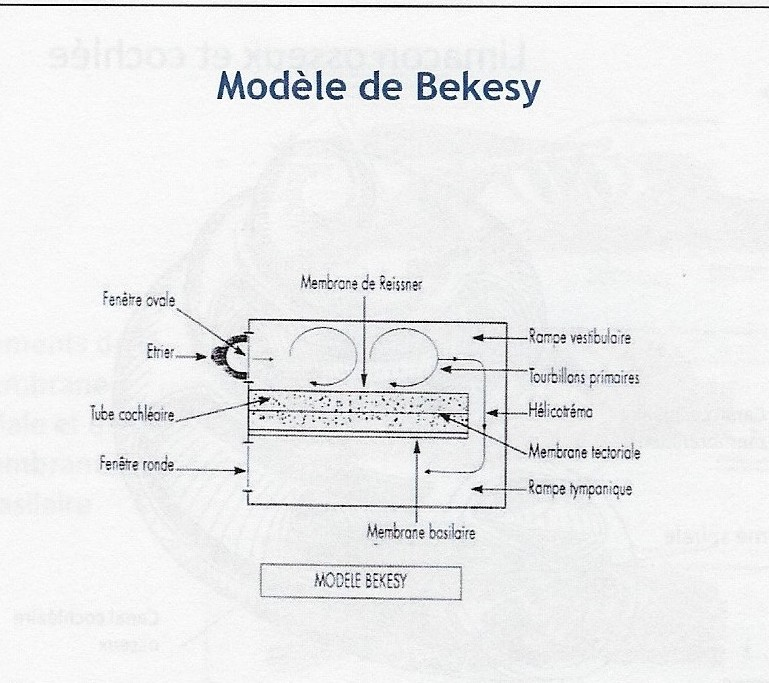
\includegraphics[width=0.7\linewidth]{images/Cochleederoule_bas.jpg}
	\caption[Modèle de Békésy]{La chaîne ossiculaire est le véhicule du son/ 
		Tomatis Développement SA, 2012}
	\label{fig:cochleederoulebas}
\end{figure}



En divergence avec von Békésy, Tomatis oppose la conception de la
physiologie auditive comme active et non
passive.\footnote{Cf. Annexe A. 1. 1. Anatomie de l'oreille et sa physiologie}
Son originalité réside ainsi dans la transmission du son
au niveau de l'oreille moyenne et interne. Le son est conduit immédiatement en direction de l'oreille 
interne grâce à l'os périphérique qui entoure la membrane tympanique.
\begin{figure}
	\centering
	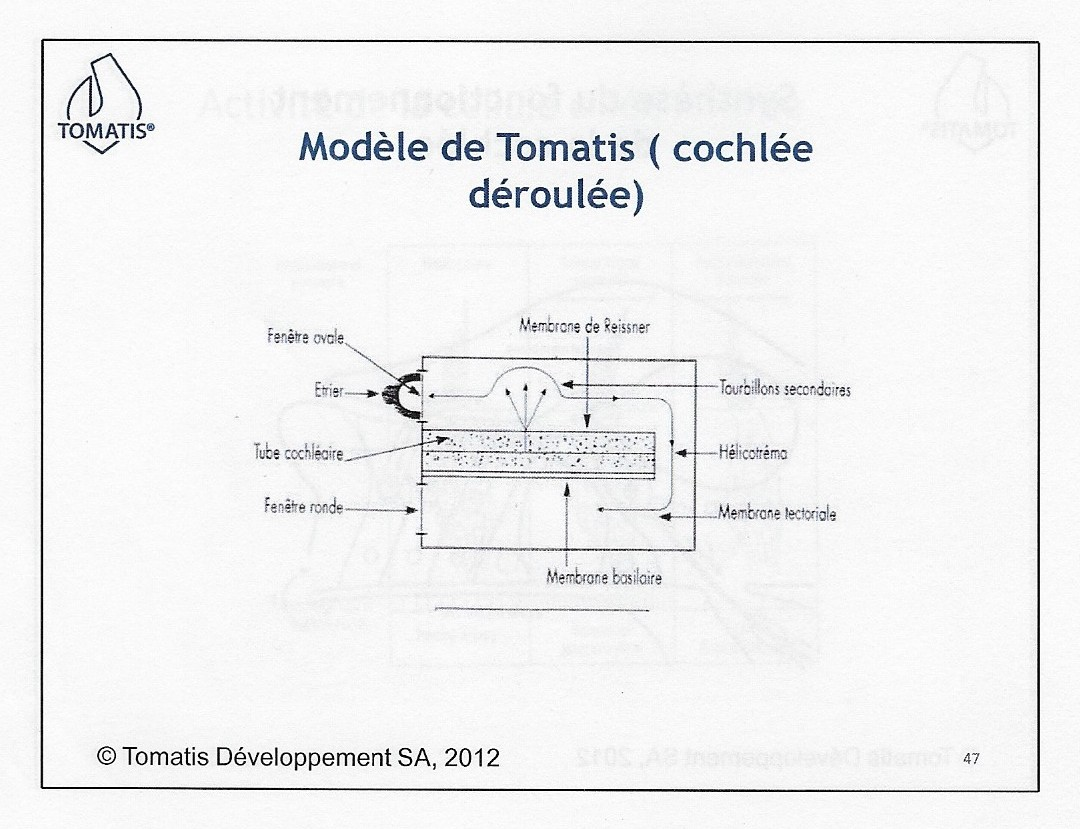
\includegraphics[width=0.7\linewidth]{images/Cochleederoule_haut.jpg}
	\caption[Cochlée selon Tomatis]{Le son passe directement  
		dans l'oreille interne et les osselets jouent un rôle de régulation, d'adaptation et non de 
		transmission.}
	\label{fig:cochleederoulehaut}
\end{figure}
\begin{quotation}
	``Le tympan se met dans un certain état de tension pour jouer le
	rôle d'un diapason qui fait vibrer toute la boîte crânienne
	par l'intermédiaire du sulcus tympani.
	C'est toute la boîte crânienne qui vibre et qui transmet le son à
		la vésicule labyrinthique et non à la chaîne ossiculaire que l'on a l'habitude
		de considérer comme le véhicule du son.La chaîne ossiculaire est un ensemble
	qui
	joue le rôle d'adaptateur, de régulateur et non de transmetteur.'' \autocite {tomatis_conf1972}
\end{quotation}
\enquote {	La cochlée, de par sa grande densité, capte les sons
	et résonne comme du cristal}  \autocite {tomatis_conf1972}.
Notons que la transmission du son par l'os est extrêmement rapide, de
5000 $m/s$ et que ce rôle d'adaptation des tourbillons et non de transmission, 
est susceptible d'expliquer l'importance de  
la conduction osseuse relatée et référée dans le  test d'écoute Tomatis.
Le passage des sons différencie donc les deux conceptions énoncées 
en le mettant ainsi en lumière. 

De plus, le tympan, dans son rôle de transmetteur dans l'oreille
          moyenne, effectue --grâce aux muscles de l'étrier et du marteau--
		un travail de visée en ciblant les sons. Il
se tend
		pour se mettre en résonance avec les sons à percevoir.
               Il fait aussi un autre travail qui est celui de sélectionner des
sons
		pour se protéger. Ainsi le tympan se tend et se détend,
              amortit et adapte
l'intensité
		sonore inondant  l'oreille interne. Cette sélection pour se  protéger rejoint et consolide ce que nous 
		évoquions plus haut à propos des 
distorsions et du pouvoir protecteur du cerveau.

%Cette hypothèse de Tomatis semble s'ajuster actuellement avec celle 

%On pourrait aussi rajouter  l'analyse
 %        fréquentielle que fait Tomatis au niveau de la\textbf{ cochlée}:
%l'onde acoustique arrivant par le canal auditif
%jusqu'au tympan  excite la membrane tympanique, donc l'os de la caisse
%du tympan \autocite {tomatis_conf1972}.%auriol:cle
%\enquote {A l'instar d'une
%peau de tambour qui fait chanter le bois auquel elle est attachée,
%c'est toute la boîte crânienne qui est inondée de sons et en particulier
%l'oreille interne. La cochlée, de par sa grande densité, capte les sons
%et résonne comme du cristal.} Notons bien que la transmission du son par l'os est de
%5000 $m/s$.
%Les fréquences qui forment les sons vont ainsi exciter les cellules
%ciliées la tapissant, tel un piano enroulé.
%Chaque fréquence se dirige \textbf{instantanément }et
%naturellement vers la cellule ciliée correspondante grâce à la
%forme du limaçon, produisant ainsi un tri fréquentiel
%instantané.


%, dans un entretien (2012),
%réalisé par Laurent Salters et Vincent Gaullier, basé sur la revue
%\textit{``Look at science''}\,>>}
%Le rôle des tourbillons est de \textbf{s'adapter aux bruits}
%et non de transmettre les sons.
%Lorsque l'intensité des sons aug\-men\-te,
%l'ex\-ci\-ta\-tion des cellules ciliées provoque des perturbations liquidiennes
%dans l'oreille interne, c'est-à-dire des tourbillons. Ceux-ci se propagent
%et sont amortis par l'étrier. Si les sons atteignent une intensité
%dangereuse pour les cellules ciliées, l'étrier réagit fortement et
%entraîne une réaction du marteau qui modifie la tension du tympan.
%A son tour, le tympan, relâché, amortit le volume sonore transmis
%à l'oreille interne, comme la paupière qui se ferme quand la lumière
%est trop intense.
Par ce rapide survol, nous constatons que  le 
chemin 
parcouru par 
le son s'explique avec différentes théories  dont celles de von Békésy et 
Tomatis. Il ne nous appartient pas de prendre le parti de l'un ou de l'autre, mais de comprendre 
davantage les bases d'une approche  et de les situer  afin de définir  le 
contexte dans lequel le test d'écoute s'est construit.
% C'est ce qui nous intéresse avant tout. 
Il est à 
remarquer que l'énigme du 
rôle de la cochlée persiste encore et toujours, l'audition restant 
sujet de grandes 
recherches dont celles menée par Christine Petit\footnote{Christine Petit, titulaire de la 
	chaire Génétique et
	Physiologie cellulaire au Collège de France} et son équipe (2012, 
2019) %Même si le rôle de la cochlée reste encore mystérieux, 
qui relève que 
\nomenclature{cochlée}{Anatomie : organe de l'audition, appareil sensoriel,
	en forme de spirale, la cochlée, incluse dans l'os du rocher,
	forme le limaçon membraneux, se situe dans l'oreille interne et
	permet de déceler des sons extrêmement faibles, de discriminer des fréquences
	et de masquer des sons faibles par des sons forts.}
<<\,c'est une sorte de minuscule appareil électroacoustique capable
de discréminer des sons extrêmement faibles, capable de masquer
	les sons faibles par des sons forts, pouvant distordre les
	sons,et capable d'élaborer un traitement extrêmement
	sophistiqué des sons``. \,>> \autocite{petit_lookscience}.%  \footnote{Christine Petit, titulaire de la 
%	chaire Génétique et
%	Physiologie cellulaire au Collège de France}

%Avant de poursuivre sur l'explication de la technique du test, nous aimerions faire l'observation 
%suivante:
%Il  n'y  a pas de conflit d'intérêt. Nous utilisons le test comme outil.
%le test d'écoute est un outil indéniable, très riche dans son apport d'informations sur la modification de 
%l'écoute, confirmée par la valeur des recherches de Tomatis. Néanmoins, nous restons très critique: la 
%transparence est un mot d'ordre en science; cela devrait être aussi le cas dans cette méthode. 
%Nous ne pouvons que le regretter.
%les chiffres  de la calibration du test qui devrait être 
%divulgué et appartenir au domaine publique
%comme dans toutes recherches scientifiques. Ce manque de clarté est regrettable.
%De plus, il  y a eu beaucoup de 
%polémique autour du personnage, de la personnalité.
%, ce qui lui enlève une certaine crédibilité. 
%le personnage....  Malgré tout, ceci ne nous empêche pas de porter un

 




%Somme toute, on peut penser que Tomatis a été très à l'avant-garde
%dans ses recherches.

%D'autres études récentes prouvent l'effet anxiolytique lors de
%l'application de cette
%méthode Tomatis\footnote{\emph{Tomatis Research and Publication} www.tomatisassociation.org}  avec Flehming
%I., 1996 \footnote{Dr. med. Inge Flehming,
%	neurologue, neuropédiatre \emph{``Grundsatz-Gutachten zur Behandlungsmethode
%		nach Prof. Tomatis''}. Voir
%\href{http://www.analytische-hoertherapie.de/uploads/tx\_templavoila/Grundsatzgu
%tachten\_zur\_Behandlungsmethode\_nach\_Prof.\_Tomatis.pdf}{le site
%web.}} et Du Plessis W. F. and Van Jaarsveld P. E., 1988.
% \footnote{Du Plessis W. F. and Van Jaarsveld P. E. ,1988, \textit{``Troubles
%psychologiques''} (Université de Potchefstroon
%- Afrique du Sud).
	%\textit{``Audio-psycho-phonology : A comparative outcome study on anxious
%primary school pupils'''},  Afr. Tydskr. Sielk. 19818 (4) 144--151. Du Plessis, W.F., Burger, S. (2001) [\ldots]
%	\emph{A pilot study involving the Tomatis method.}, Sud Africa J.
%Psychol.}
